\chapter{Requirements, Constraints and Design}

In this chapter we will talk about the design of the bootware component and the requirements and constraints that shape it.
We begin with the requirements, which were explicitly given at the beginning of the thesis.
Next, we describe additional constraints which we added to limit the scope of the work.
Then, we explain the design that formed as a result of the limitations that we had.

\section{Requirements}

The main goal of this diploma thesis is to lay a foundation by creating the core design of the bootware.
It was clear from the beginning that, because of the limited time available, not every feature that might be necessary for the full operation can be fully implemented.
Instead, the foundation we develop here should keep future needs in mind and make it simple to extend the bootware when needed.
It is therefore a core requirement to keep the bootware relatively generic and make it extensible where necessary.

It should be extensible in two key areas, namely the support for different cloud providers and for different provisioning engines.
For this diploma thesis, Amazon is the only cloud provider that has to be supported, but it has to be possible to add others in the future.
Concerning provisioning engines, only OpenTOSCA has to be supported for now, but again with the possibility to add more in the future.

It is also important that the bootware is easy to use.
In fact, it should be practically invisible whenever possible.
It should hook into the already existing process of executing a workflow without adding unnecessary interaction steps when possible.
However, It cannot be hidden completely, because the user has to specify a cloud provider and the corresponding log-in credentials somewhere.
The user should also get some feedback about the progress of the deployment because this process might take some time and might seem unresponsive without frequent status updates.

A further requirement is that the bootware should be relatively lightweight and open standards should be used where possible.
In this case, lightweight means that the bootware should be small, independent program that does not require a huge supporting infrastructure to be executed.
It should also be easy to distribute and setup and it has to be able to run on an average personal computer.

\section{Constraints}

The bootware could theoretically be written in any major programming language but we limit our selves to Java.
The reason for this is that all the other SimTech components are written in Java, so by also using Java we fit nicely into this already existing ecosystem.
Additionally, for things like Eclipse integration we would have to use Java anyway.
We also have to keep in mind that the bootware will not be finished with this thesis.
Other people will have to extend it in the future and since Java is common in general, as well as in the SimTech project, it makes sense to use it instead of another programming language.
We can further narrow our use of Java by limiting us to Java 1.6.
This also has to do with the already existing parts of the SimTech project, that are geared towards this version as well.
Using another version of Java could lead to unforeseen incompatibilities.
We also constrain the bootware usage to one bootware per user.
We don't plan for multi-tenancy, i.e. multiple users using the same bootware.
In the next chapter we will also introduce additional constraints that became necessary during the design process and will therefore be explained at the appropriate times.


\section{Design}

In this section we will develop the design of the bootware.
This design is held intentionally abstract.
Specific implementation details will be selected and described in \autoref{selecting}.

\subsection{Component Division}

The first question that has to be answered is whether or not it makes sense to divide the bootware component into two or more cooperating components, i.e. a server client division or a similar structure.
\textcolor{red}{As described in \autoref{related:ondemand} on page \pageref{related:ondemand}, the proposed architecture initially only envisioned one bootware component.
This architecture was expanded with the introduction of the provisioning manager, as described in \autoref{related:dynamic} on page \pageref{related:dynamic}.}
We will now discuss the viability of these architectures.

\subsubsection{Single Local Component}

\begin{figure}[!htbp]
	\centering
	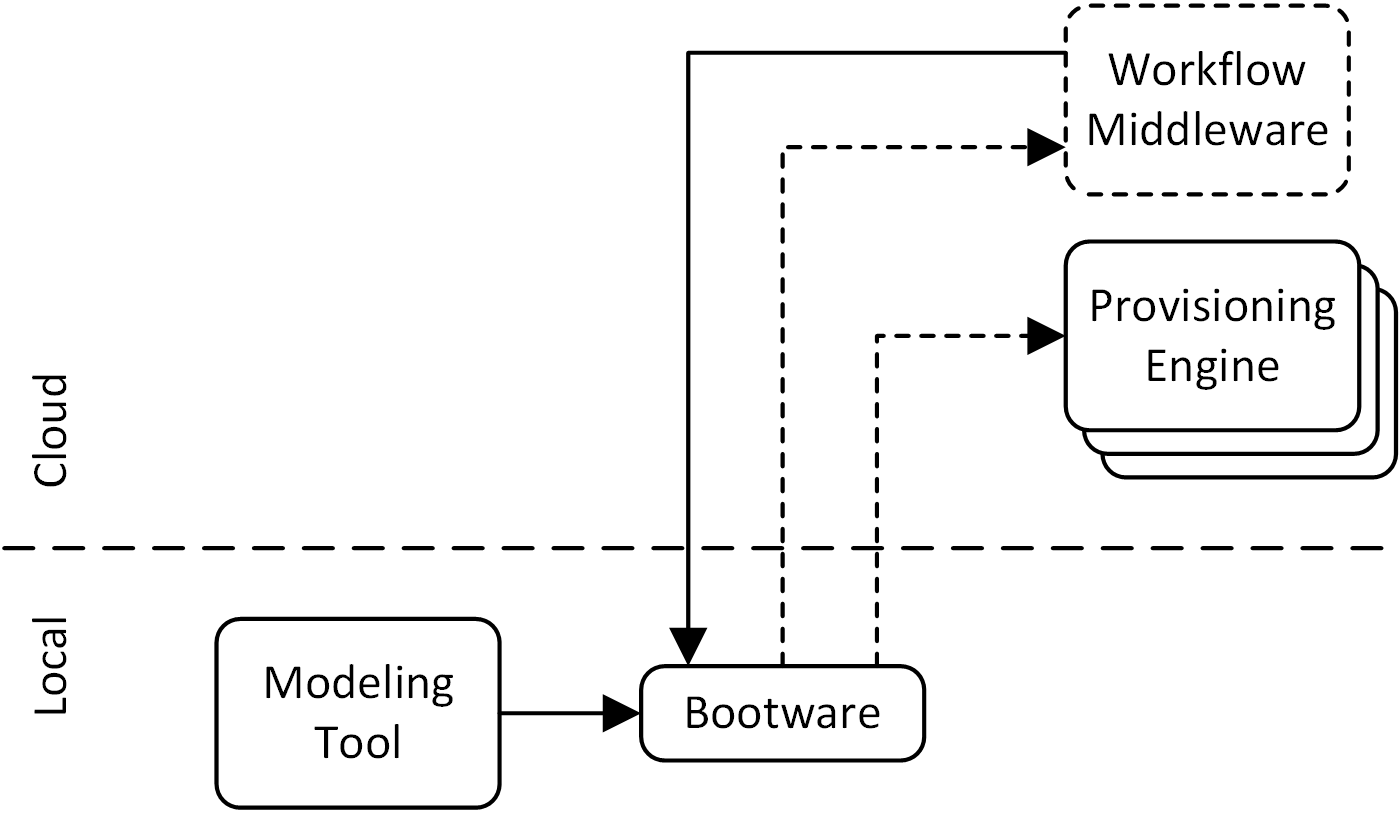
\includegraphics[resolution=600]{design/assets/simple_local}
	\caption{Simplified overview of the single local component architecture}
	\label{image:single_local}
\end{figure}

First we consider the simplest case: A single local component.
In this scenario, all provisioning processes are initiated from a component installed locally on the users machine, alongside or as part of the workflow modeler.

The advantages of this architecture lie in its simplicity.
Only one component has to be created and managed.
We wouldn't have to deal with any cloud environments and each user would have his own personal instance, so multi-tenancy wouldn't be an issue.
There is no possible overlap in functionality, as in a 2-tier architecture (see \autoref{design:division:2tier}) and communication between multiple bootware components doesn't have to be considered.

The disadvantages are caused by the component being local.
Since all the functionality is concentrated in one component, it can become quite large and complicated, which is one thing that should be avoided according to the requirements.
A much bigger problem however is the remote communication happening in this scenario.
All calls to the bootware component from the ESB of the workflow middleware would leave the remote environment.
Also, all calls from the bootware component to the provisioning engines would enter the remote environment.
This type of split communication can be costly and slow, as shown by Li et al.
They compared public cloud providers and measured that intra-datacenter communication can be two to three times faster and also cheaper (often free) compared to inter-datacenter communication~\autocite{cloudcmp}.

\subsubsection{Single Remote Component}

\begin{figure}[!htbp]
	\centering
	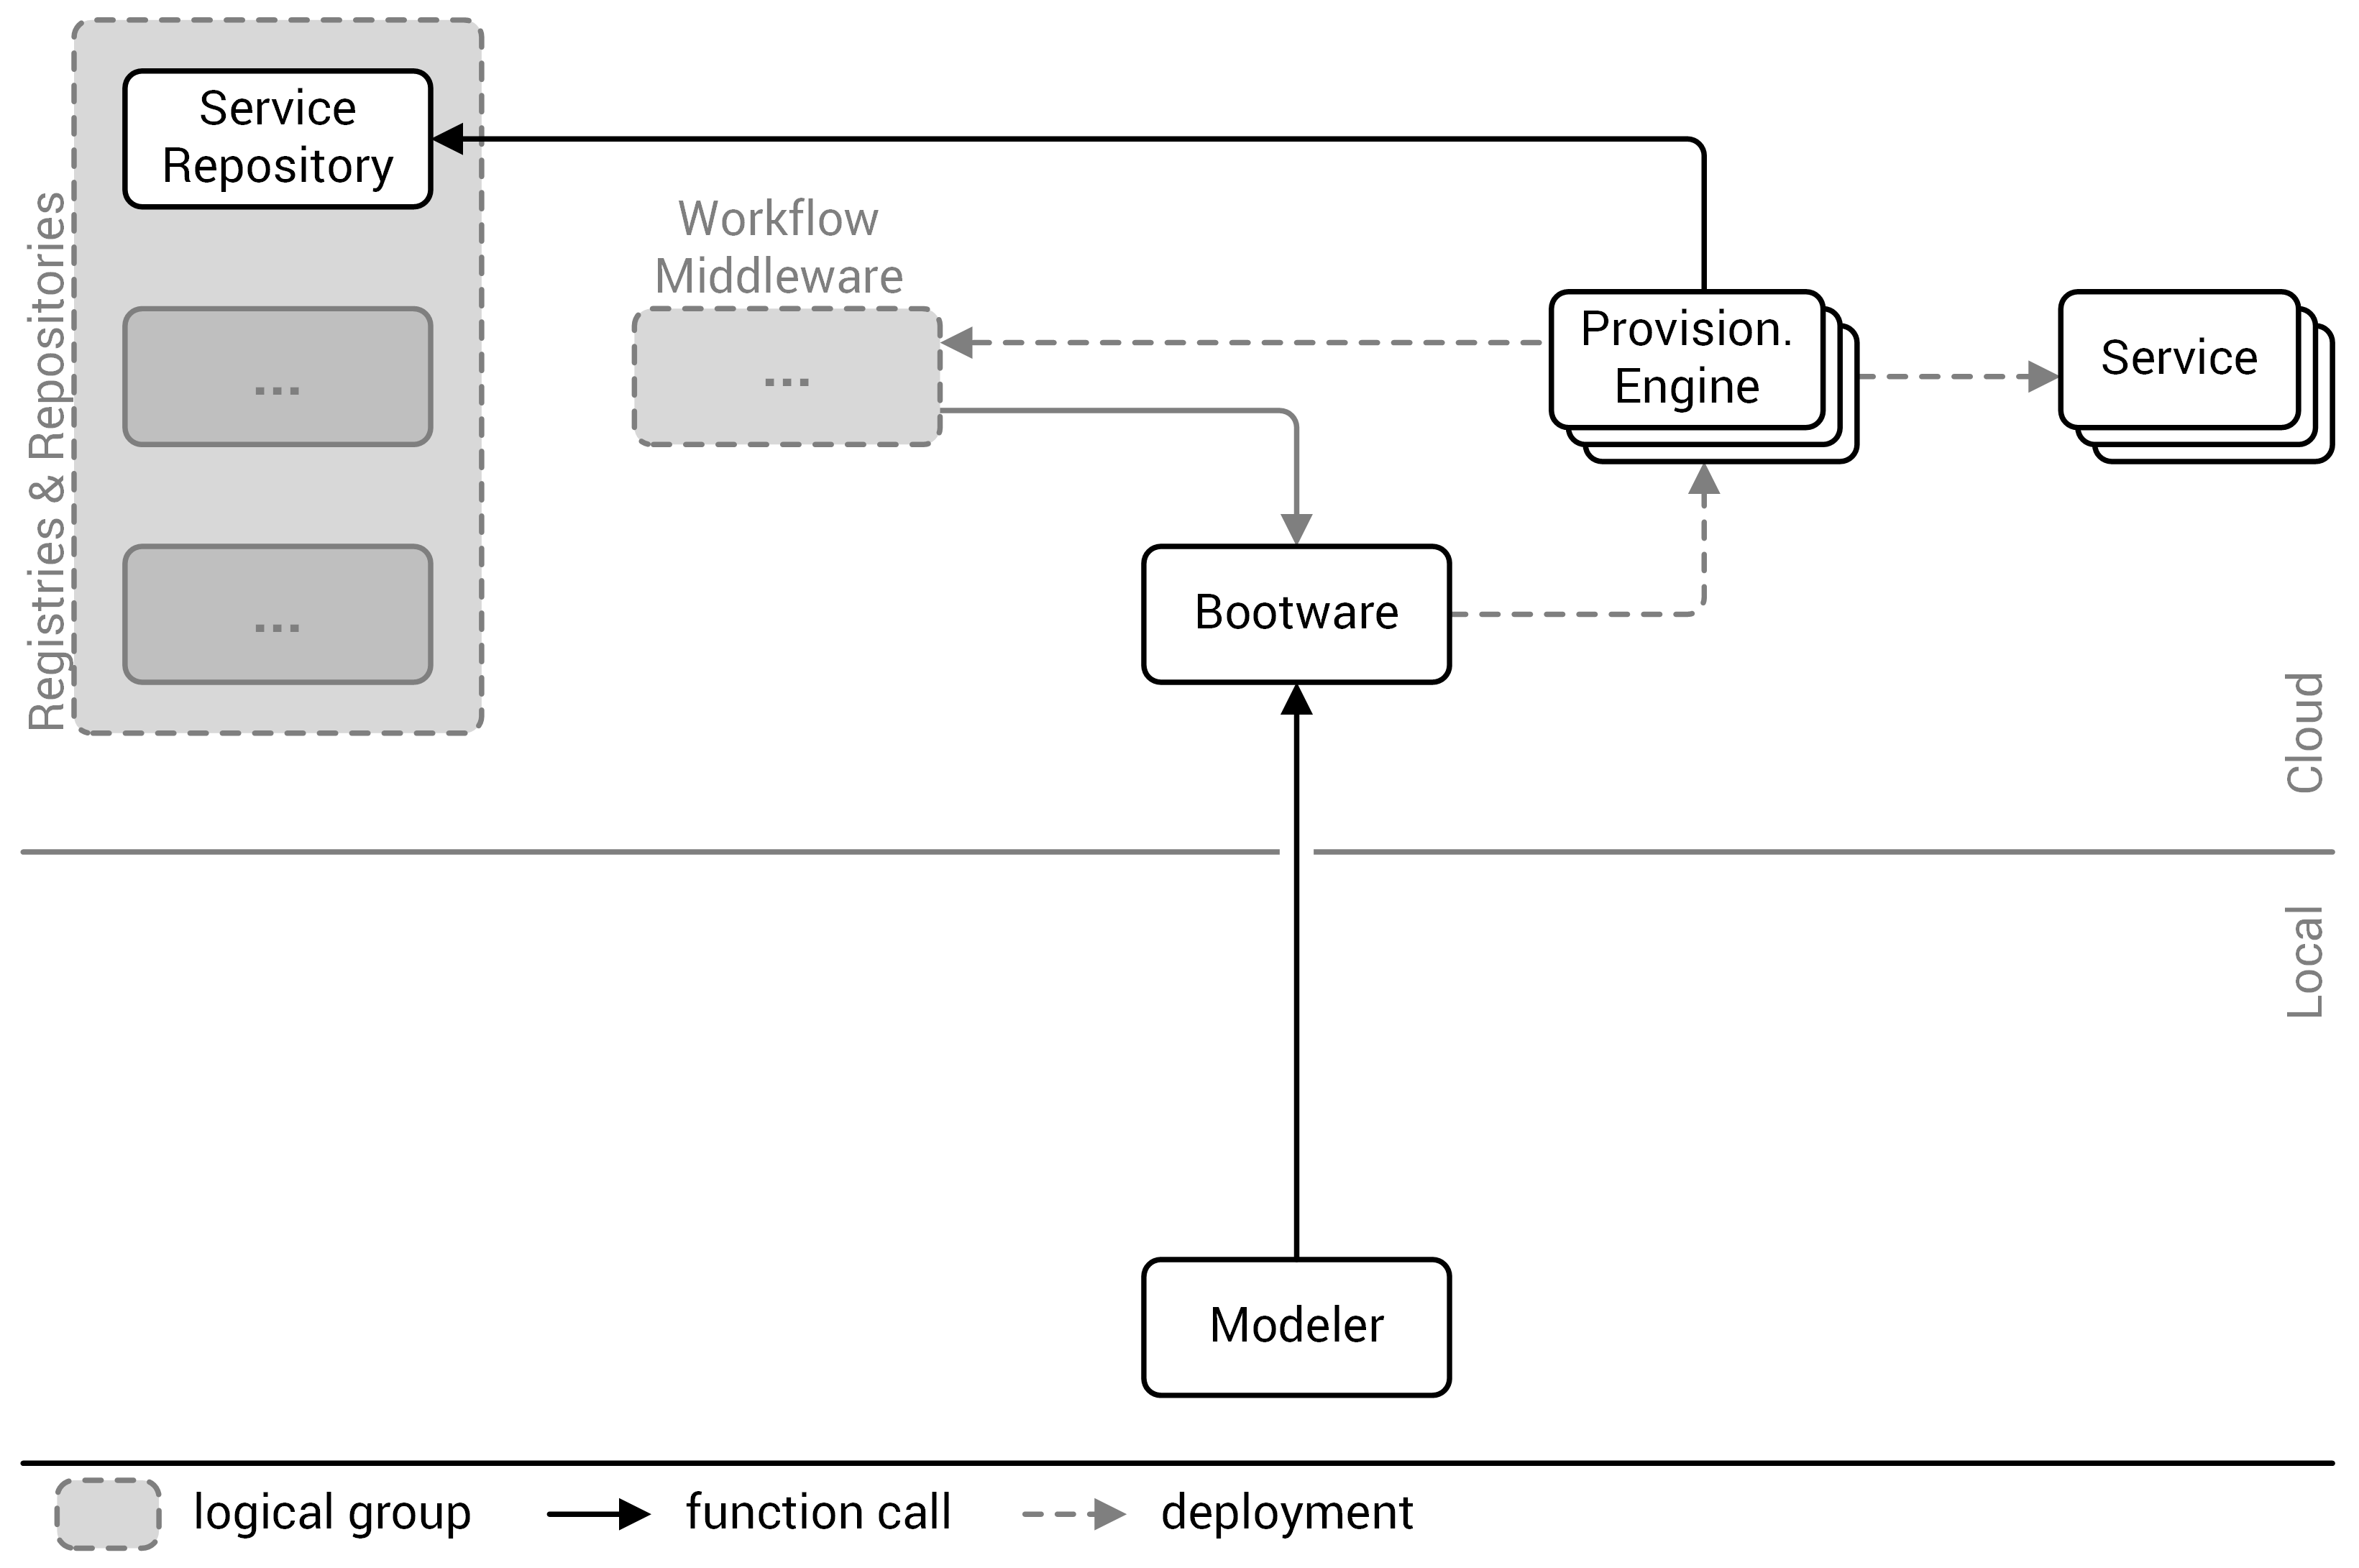
\includegraphics[resolution=600]{design/assets/simple_remote}
	\caption{Simplified overview of the single remote component architecture}
	\label{image:single_remote}
\end{figure}

The next obvious choice is to put the single bootware component into a remote environment, where the disadvantages of local to remote communication would disappear.
However, this creates new problems.

Since there aren't any additional components in this scenario that could manage the life-cycle of the remote bootware, the user would have to manage it by hand, which leads to two possibilities.
Either the user provisions the bootware once in some cloud environment and then keep this one instance running or she provision it once she needs it and deprovisions it when she is done.

In the first case the user would only have to provision the bootware once, but this creates a new problem: The user doesn't know where exactly to put the bootware component.
Since one requirement is that multiple cloud environments should be supported, it's possible that the bootware component is not located anywhere near the cloud environment where it should provision further components.
The communication problem of the single local bootware component can still occur in these cases.

Another problem is that the bootware would be running all the time, even if the user doesn't need it, which would increase costs.
This problem could be reduces if this bootware instance is shared with others to assure a more balanced load.
But then the user would have to manage some sort of load balancing and the bootware component would have to support multi-tenancy or be stateless to be able to cope with potential high usage spikes.
This would further complicate the design and implementation of the bootware component and possibly increase the running costs.

In the second case the user would provision the bootware whenever she needs it.Now the user would be able to pick a cloud environment that is close to the other components that she plans to provision later.
This eliminates the two major problems of the first case but increases the effort that the user has to put into a task that she shouldn't have to do in the first place.
Life-cycle management of the bootware should be automated completely and hidden away from the user.
Therefor, this scenario is not appropriate for our case.

\subsubsection{2-Tier Architecture}
\label{design:division:2tier}

\begin{figure}[!htbp]
	\centering
	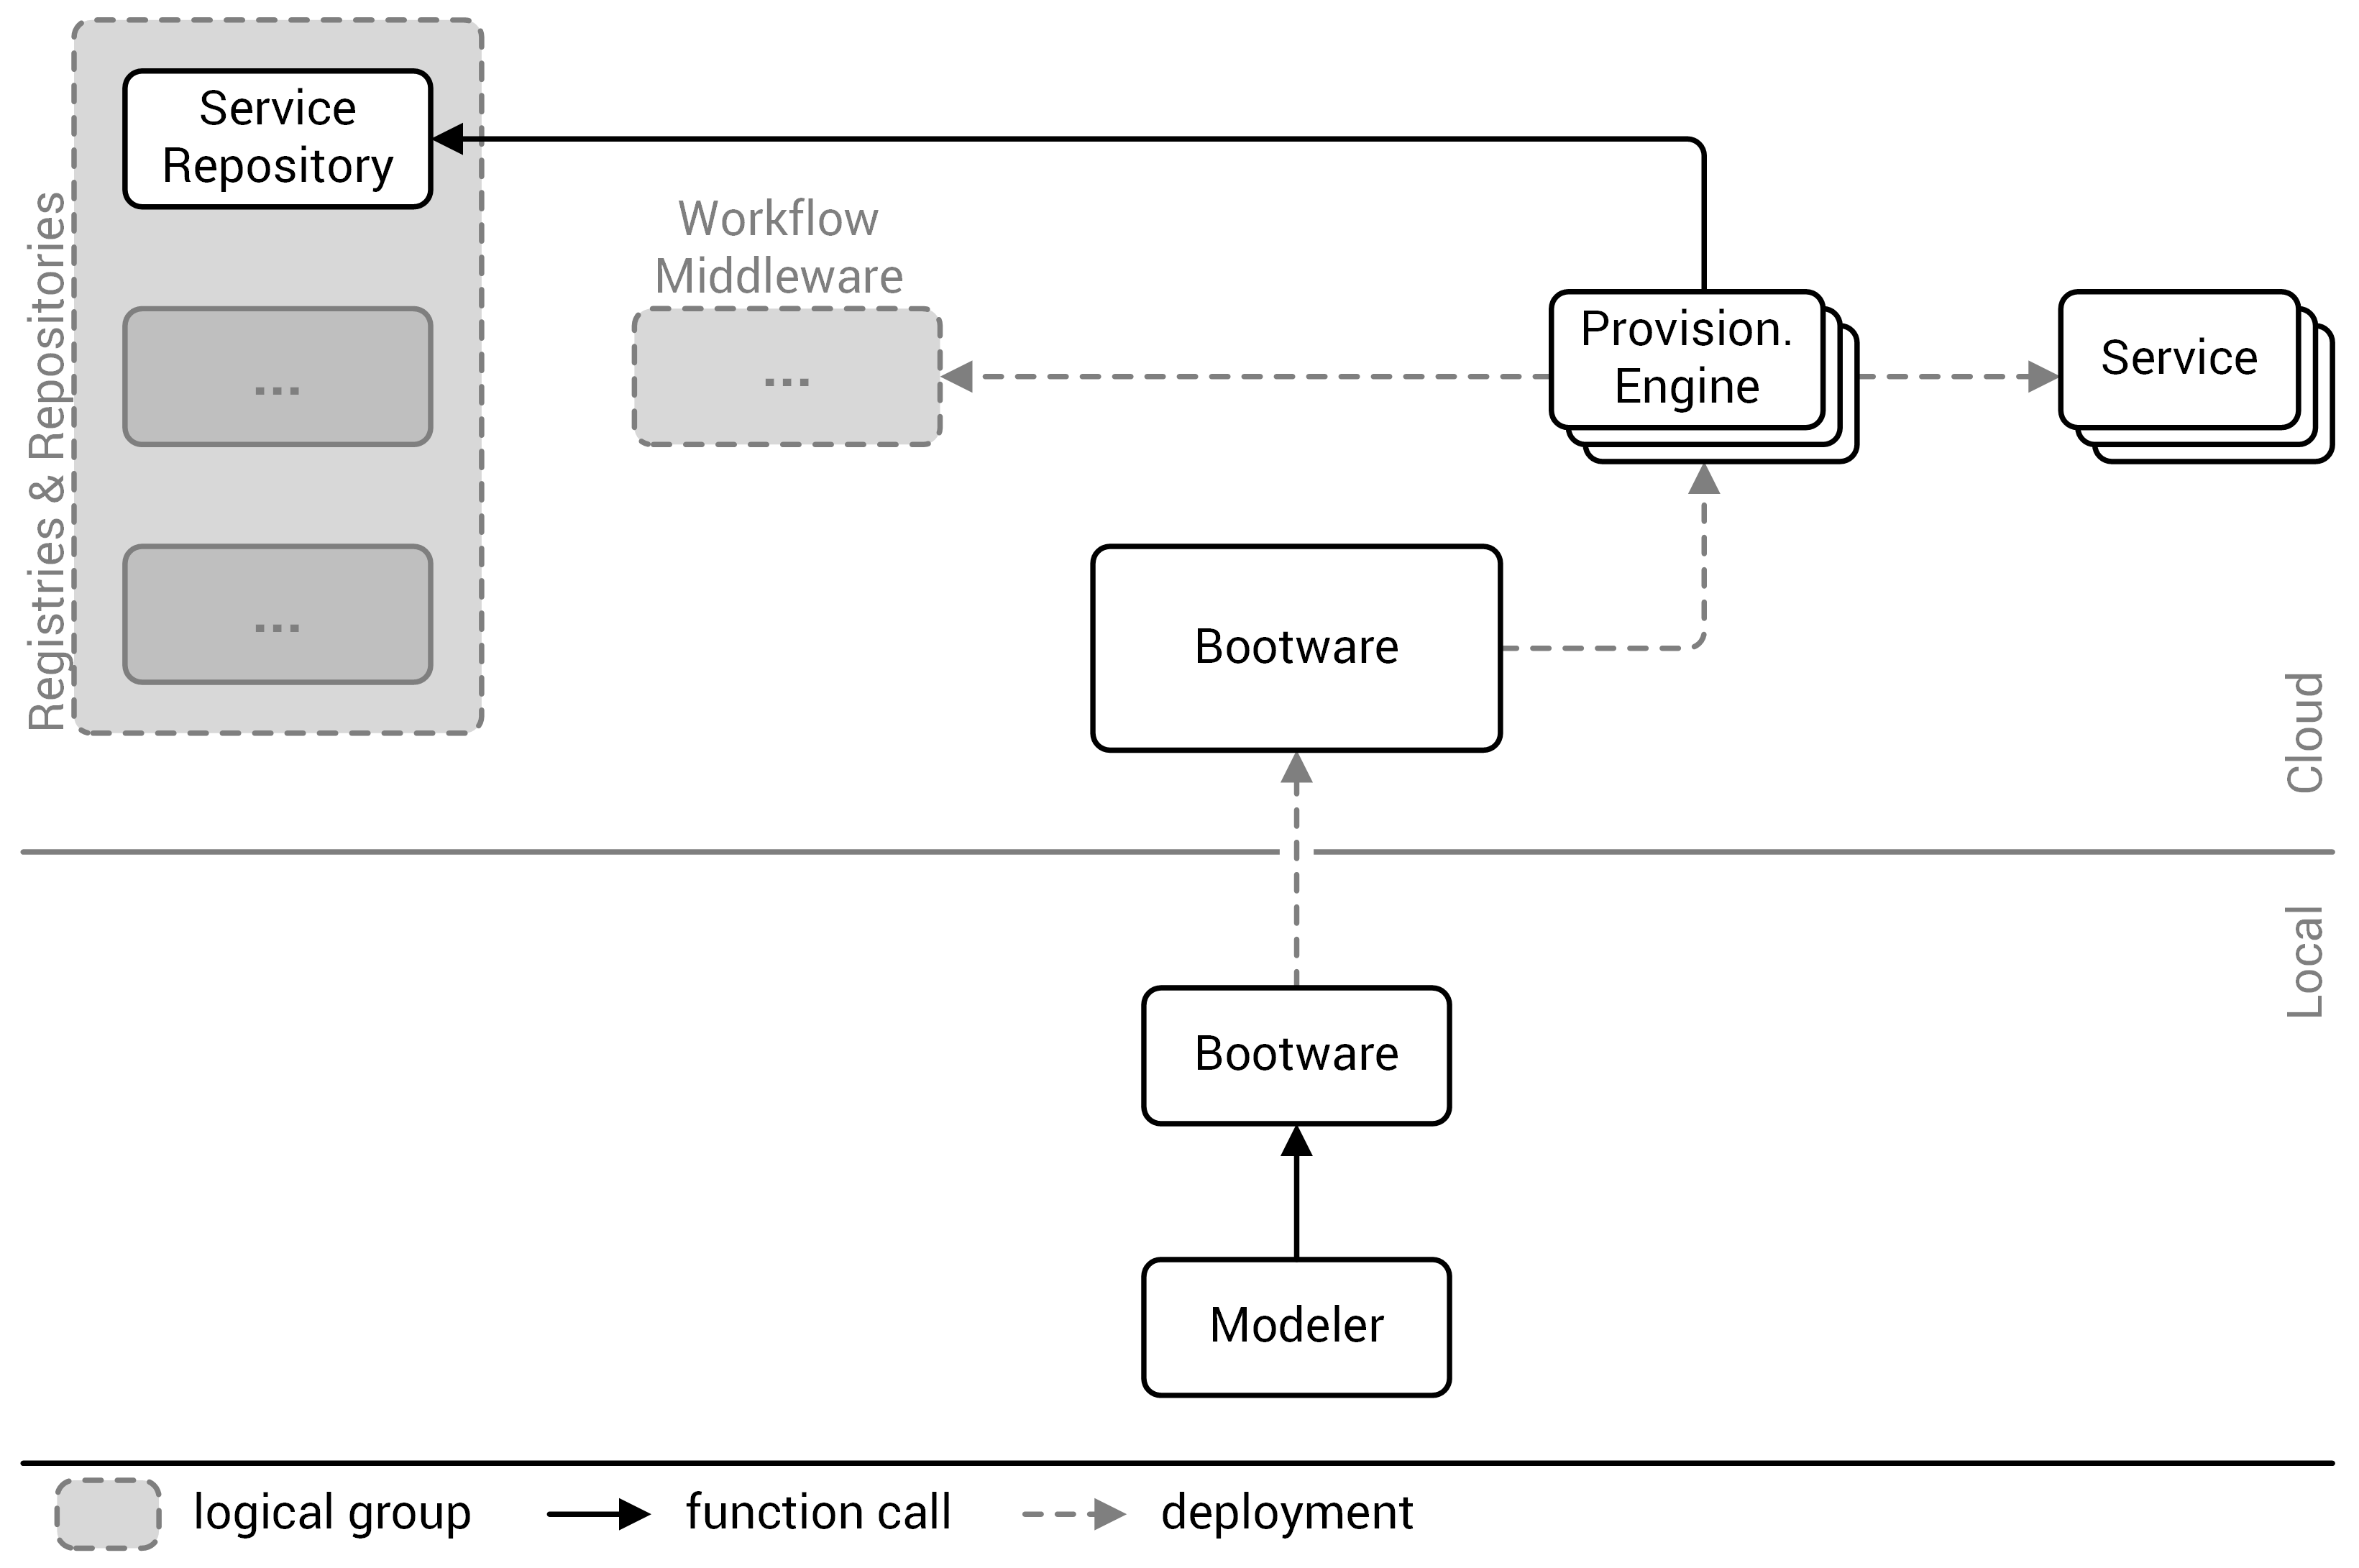
\includegraphics[resolution=600]{design/assets/simple_2_tier}
	\caption{Simplified overview of the 2-tier architecture}
	\label{image:2_tier}
\end{figure}

Next, we take a look at a 2-tier architecture, where the bootware is divided into two components.
On the local side we have a small and simple component which has mainly one function: To provision the larger second part of the bootware in a remote environment near to the environment, where other components will be provisioned later.

This eliminates the problems of a single local or remote bootware component.
The user no longer has to be involved in the management of the remote bootware since the local bootware handles all that.
Since we provision the remote bootware on demand we now also can position the remote component close to other remote components to minimize local/remote communication and the problems resulting of it.
We can now keep the local part as simple as possible and make the remote part as complicated as it has to be and since we provision the remote bootware only for one user we don't have to worry about multi-tenancy.

But we also introduce new problems.
For one, we now have duplicate functionality between the two components.
Both components have to know how to provision a component into multiple cloud environments.
The local component has to be able to put its remote counterpart into any cloud environment.
The remote component has to be able to provision other components into the same environment in which it runs (ideally, to minimize costs).
Since itself can be located in any cloud environment, it has to be able to do this in any cloud environment.
Independent from this, it has to be able to provision to any environment that the user/service package chooses.
But this problem can be solved by using a plugin architecture, which allows both components to use the same plugins.
We discuss plugins in detail in \autoref{design:extensibility}.

\textcolor{red}{A second problem which we can't avoid but can solve is the communication which is now necessary between the different parts of the bootware.
More on this in \autoref{design:communication}}

\subsubsection{Cloning}

\begin{figure}[!htbp]
	\centering
	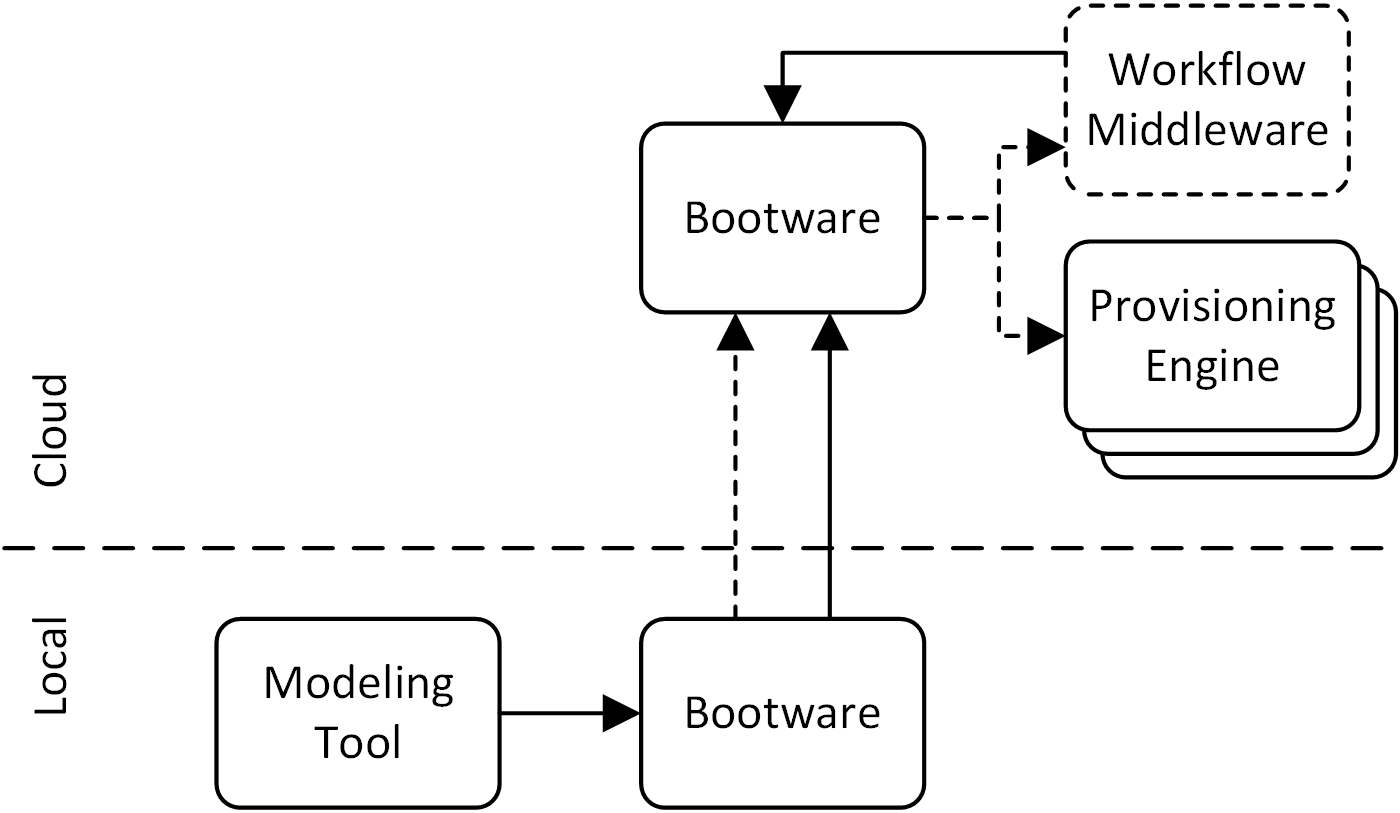
\includegraphics[resolution=600]{design/assets/simple_clone}
	\caption{Simplified overview of the cloned component architecture}
	\label{image:clone}
\end{figure}

This architecture can be seen as an alternative form of the 2-tier architecture described in \autoref{design:division:2tier}.
In this case there are also two parts working together and the remote part does most of the work.
However, the local and the remote components are identical.
Instead of provisioning a bigger component in a remote environment, the local component clones itself.
Compared to the 2-tier architecture described before, this has the advantage that only one component has to be designed and implemented and that function duplication is not an issue.
The disadvantage would be that the local bootware would be exactly as complex as the remote bootware and would contain unnecessary functionality (e.g. a web service interface).
However, since we want to keep the whole bootware, including the remote part, fairly lightweight, it's highly unlikely that the complexity of the remote bootware will reach such heights that it could not be run on an average local machine.
In this case, the advantage of only having to design and implement one component seems to outweigh the disadvantage of a slightly more complex local component (compared to the 2-tier variant).
Of course, this architecture makes only sense if the functionality of the two separate components in the 2-tier architecture turns out to be mostly identical.
Therefore we can't decide yet if this architecture should be used.

\subsubsection{Decision}

Of the four alternative presented here, alternative three - the 2-tier architecture - makes the most sense.
Therefore it is selected as the alternative of choice and used for further discussion.
We do however retain the option to transform it into alternative four if we discover that both components share much of same functionality, but this can only be judged at a later stage, when we know exactly how the internal functionality of the bootware will work.

\section{Extensibility}
\label{design:extensibility}

In \autoref{design:communication} we mentioned a secondary communication mechanism that would be best implemented in form of an extension to the bootware.
The requirements for the bootware also state that support for different cloud environments and provisioning engines should be achieved through means of software engineering.
These requirements are intentionally vague to allow for the selection of a fitting extension mechanism during the design process.
In this section we will take a look at different extension mechanisms for Java and pick the one that suits our needs best.

\subsection{Extension Mechanisms}

The simplest way to fulfill the extensibility requirement would be to create a set of interface and abstract classes to define the interfaces and basic functionality that are necessary to work with different cloud environments and provisioning engines.
These interfaces and abstract classes would then be implemented separately to support different scenarios and would be compiled, together with the rest of the application, into one executable.
At runtime, a suitable implementation would be selected and used to execute the specific functionality required at this time.

This extension mechanism is simple, but restricted by its static nature.
The entire executable has to be recompiled if any implementations are changed or added.
This may not be a problem if the set of possible extensions that have to be supported is limited and known at the time of implementation or if it changes rarely.
If the set of necessary extensions is unknown or changing from time to time, implementing new or changing existing extensions can get cumbersome because a new version of the whole software has to be released each time.
It would be far better if extensions could be implemented separately from the core bootware components and added and removed at will.

A more flexible architecture is needed, for example a plugin architecture.
Interfaces for the extension points still exist but the extension are no longer part of the main bootware components.
They are compiled separately into plugins that can be loaded into the main bootware components on the fly.
There are several possibilities to realize such an architecture.

It is certainly possible to implement a plugin framework from scratch.
An advantage of this approach would be that the design of the plugin architecture could be tailored to our use case and would be as simple or complex as needed.
But there are also several disadvantages.
For one, we would reinvent the wheel because multiple such frameworks already exist.
It would also shift resources away from the actual goal of this diploma thesis, which is designing the bootware.
Furthermore, it would require a deep understanding of the language used for the implementation (in this case Java), which is not necessarily given.
Therefore, it seems more reasonable to use one of the already existing plugin frameworks.
Which one exactly will be determined later in \autoref{implementation:selecting:pluginframeworks}.

\subsection{Plugin Repository}
\label{design:pluginrepository}

Now that we have introduced plugins we face new problems.
\autoref{image:plugins} shows the current architecture, where both bootware components use their own plugins.
If a plugin is added or updated, the user has to manually copy this plugin to the right folder of one or both of the bootware components.
Furthermore, if both components use the same plugins, which they will (for example plugins for different cloud providers), we will have duplicate plugins scattered around.
This is inefficient, probably annoying for the user and can cause errors if plugins get out of sync.

\begin{figure}[!htbp]
	\centering
	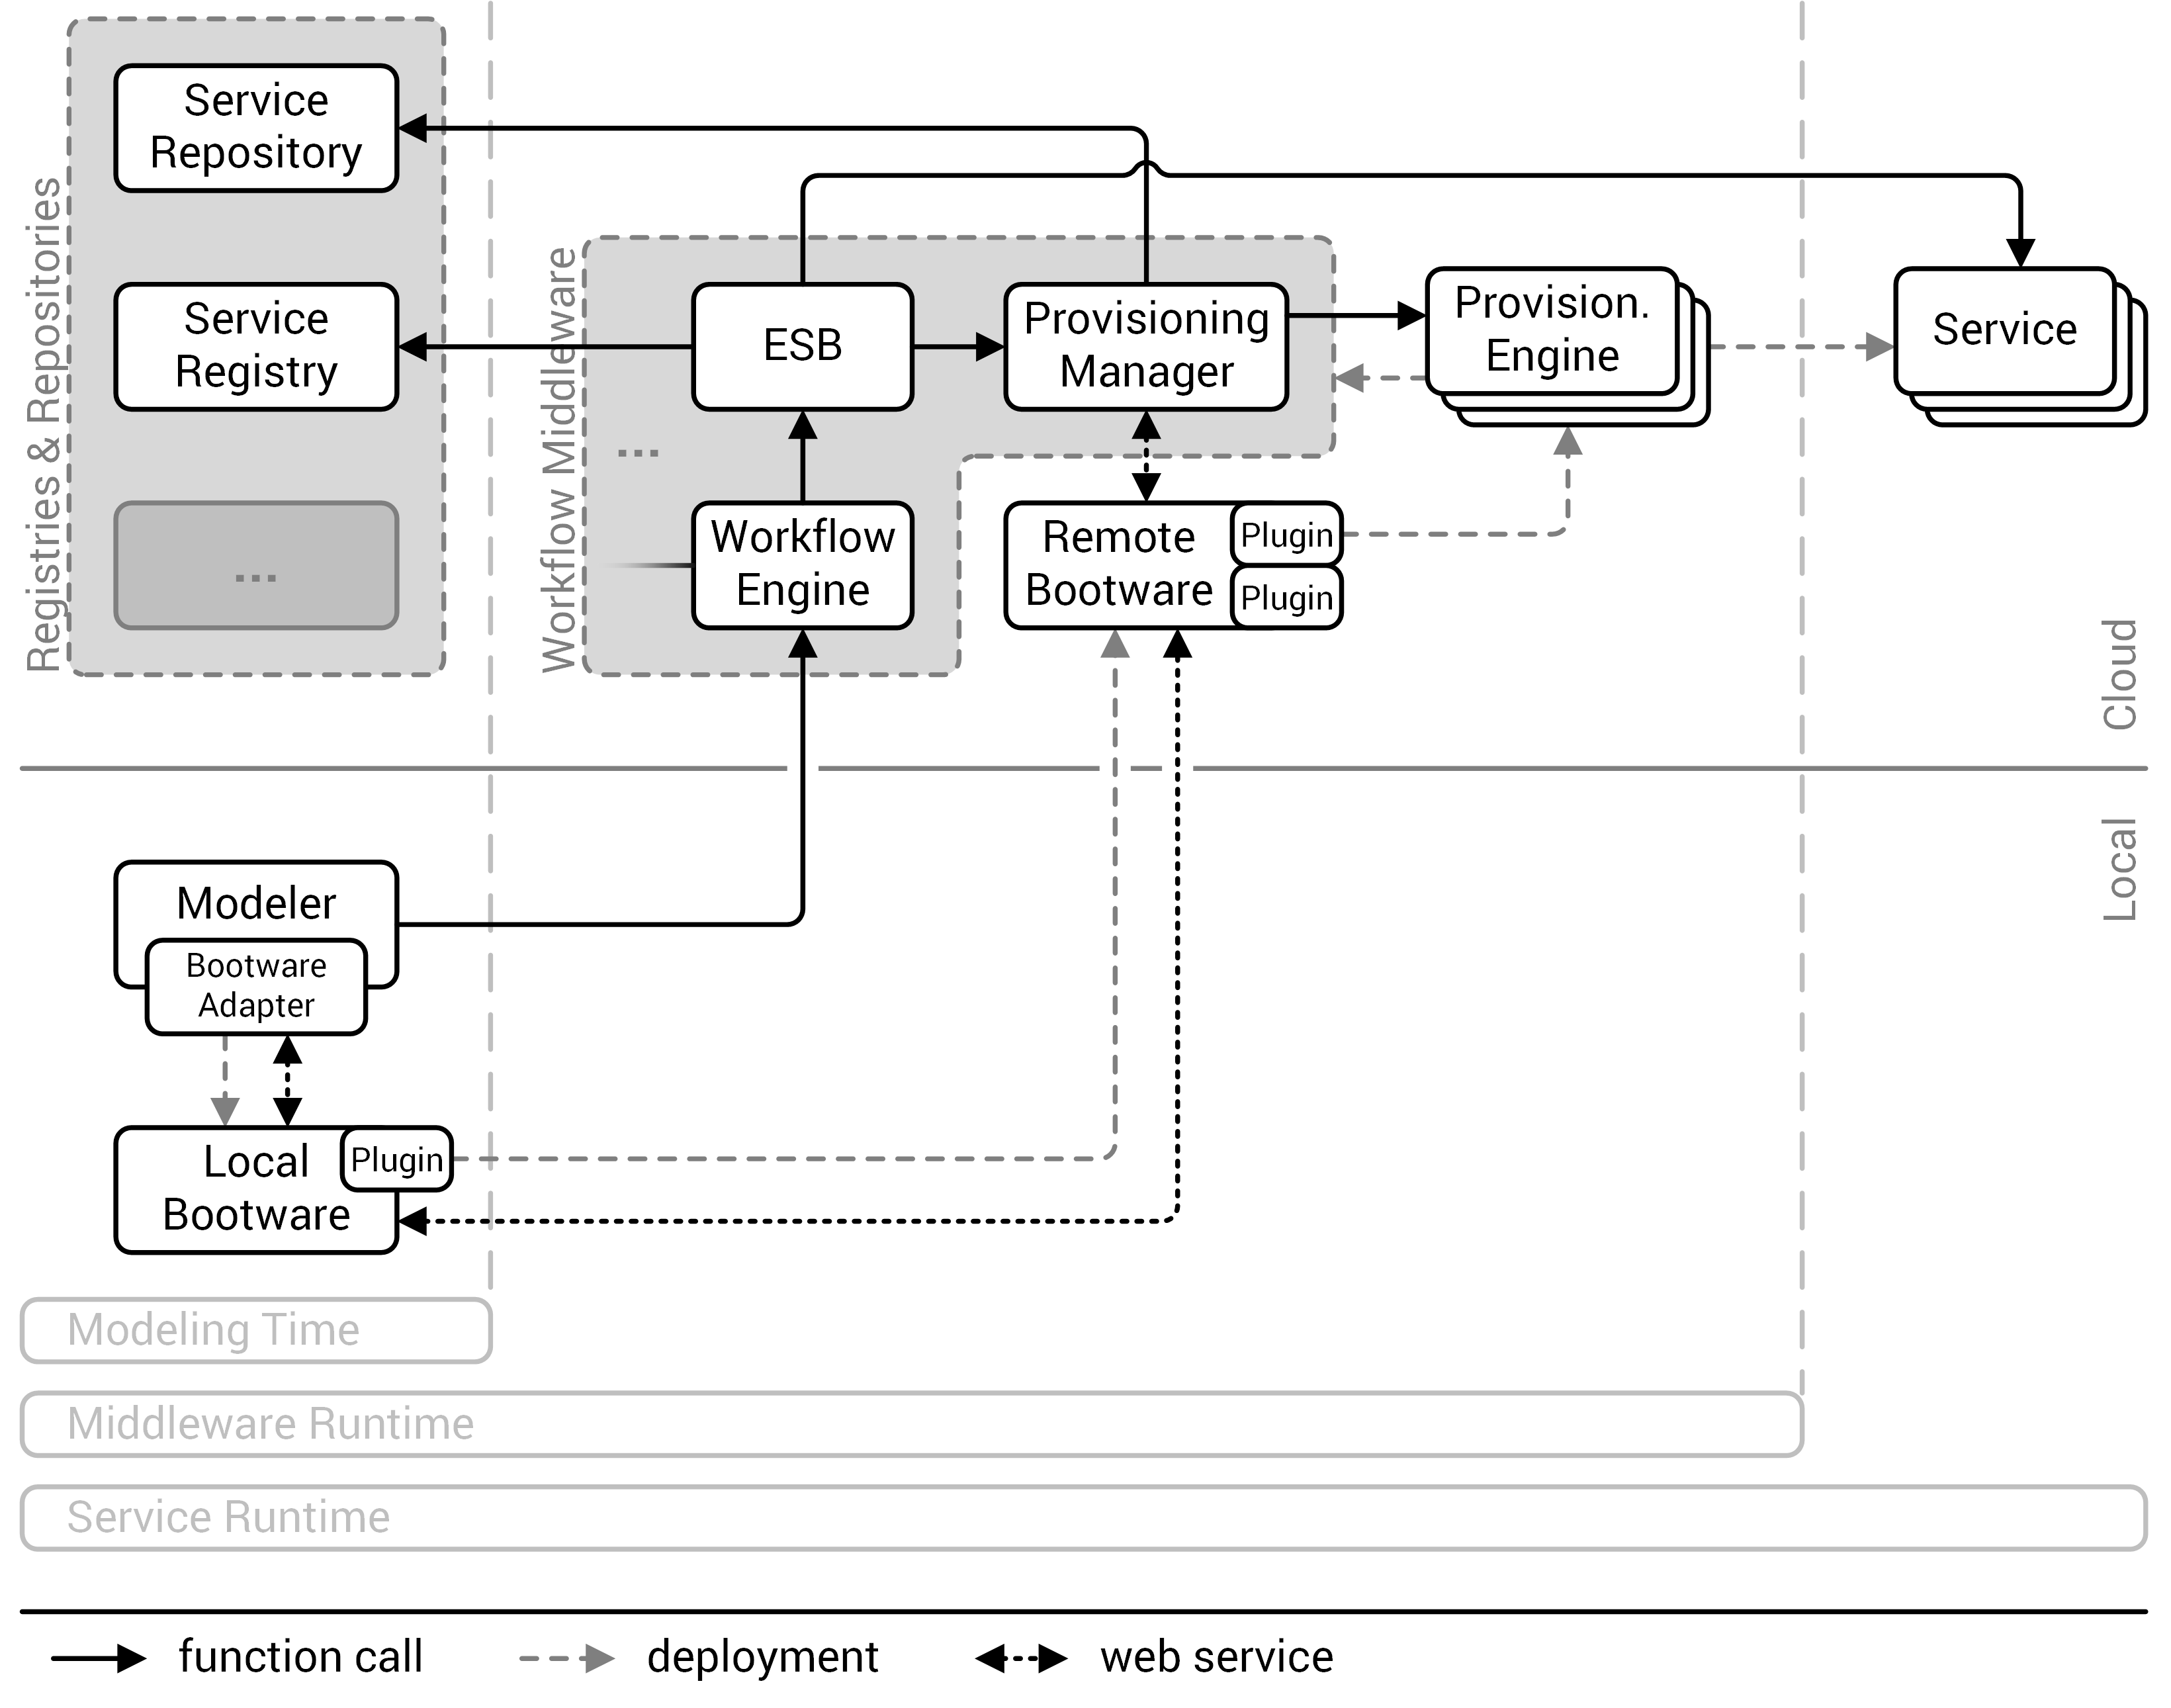
\includegraphics[resolution=600]{design/assets/plugins}
	\caption{Simplified overview of the 2-tier architecture with plugins.}
	\label{image:plugins}
\end{figure}

To remedy this situation we introduce a central plugin repository, as shown in \autoref{image:plugin_repository}.
This repository holds all plugins of both components so it eliminates duplicate plugins.
If plugins are added or modified it has only to be done in one place.
Plugin synchronization can happen automatically when the bootware components start, so that the user is no longer involved in plugin management.
The repository also enables easy plugin sharing, which was cumbersome earlier.
While a central plugin repository is a sensible addition to the proposed bootware architecture, its design and implementation are out of scope of this diploma thesis.
This work is left for the future and the plugin repository will not be mentioned in any other figures apart from \autoref{image:plugin_repository}.

\begin{figure}[!htbp]
	\centering
	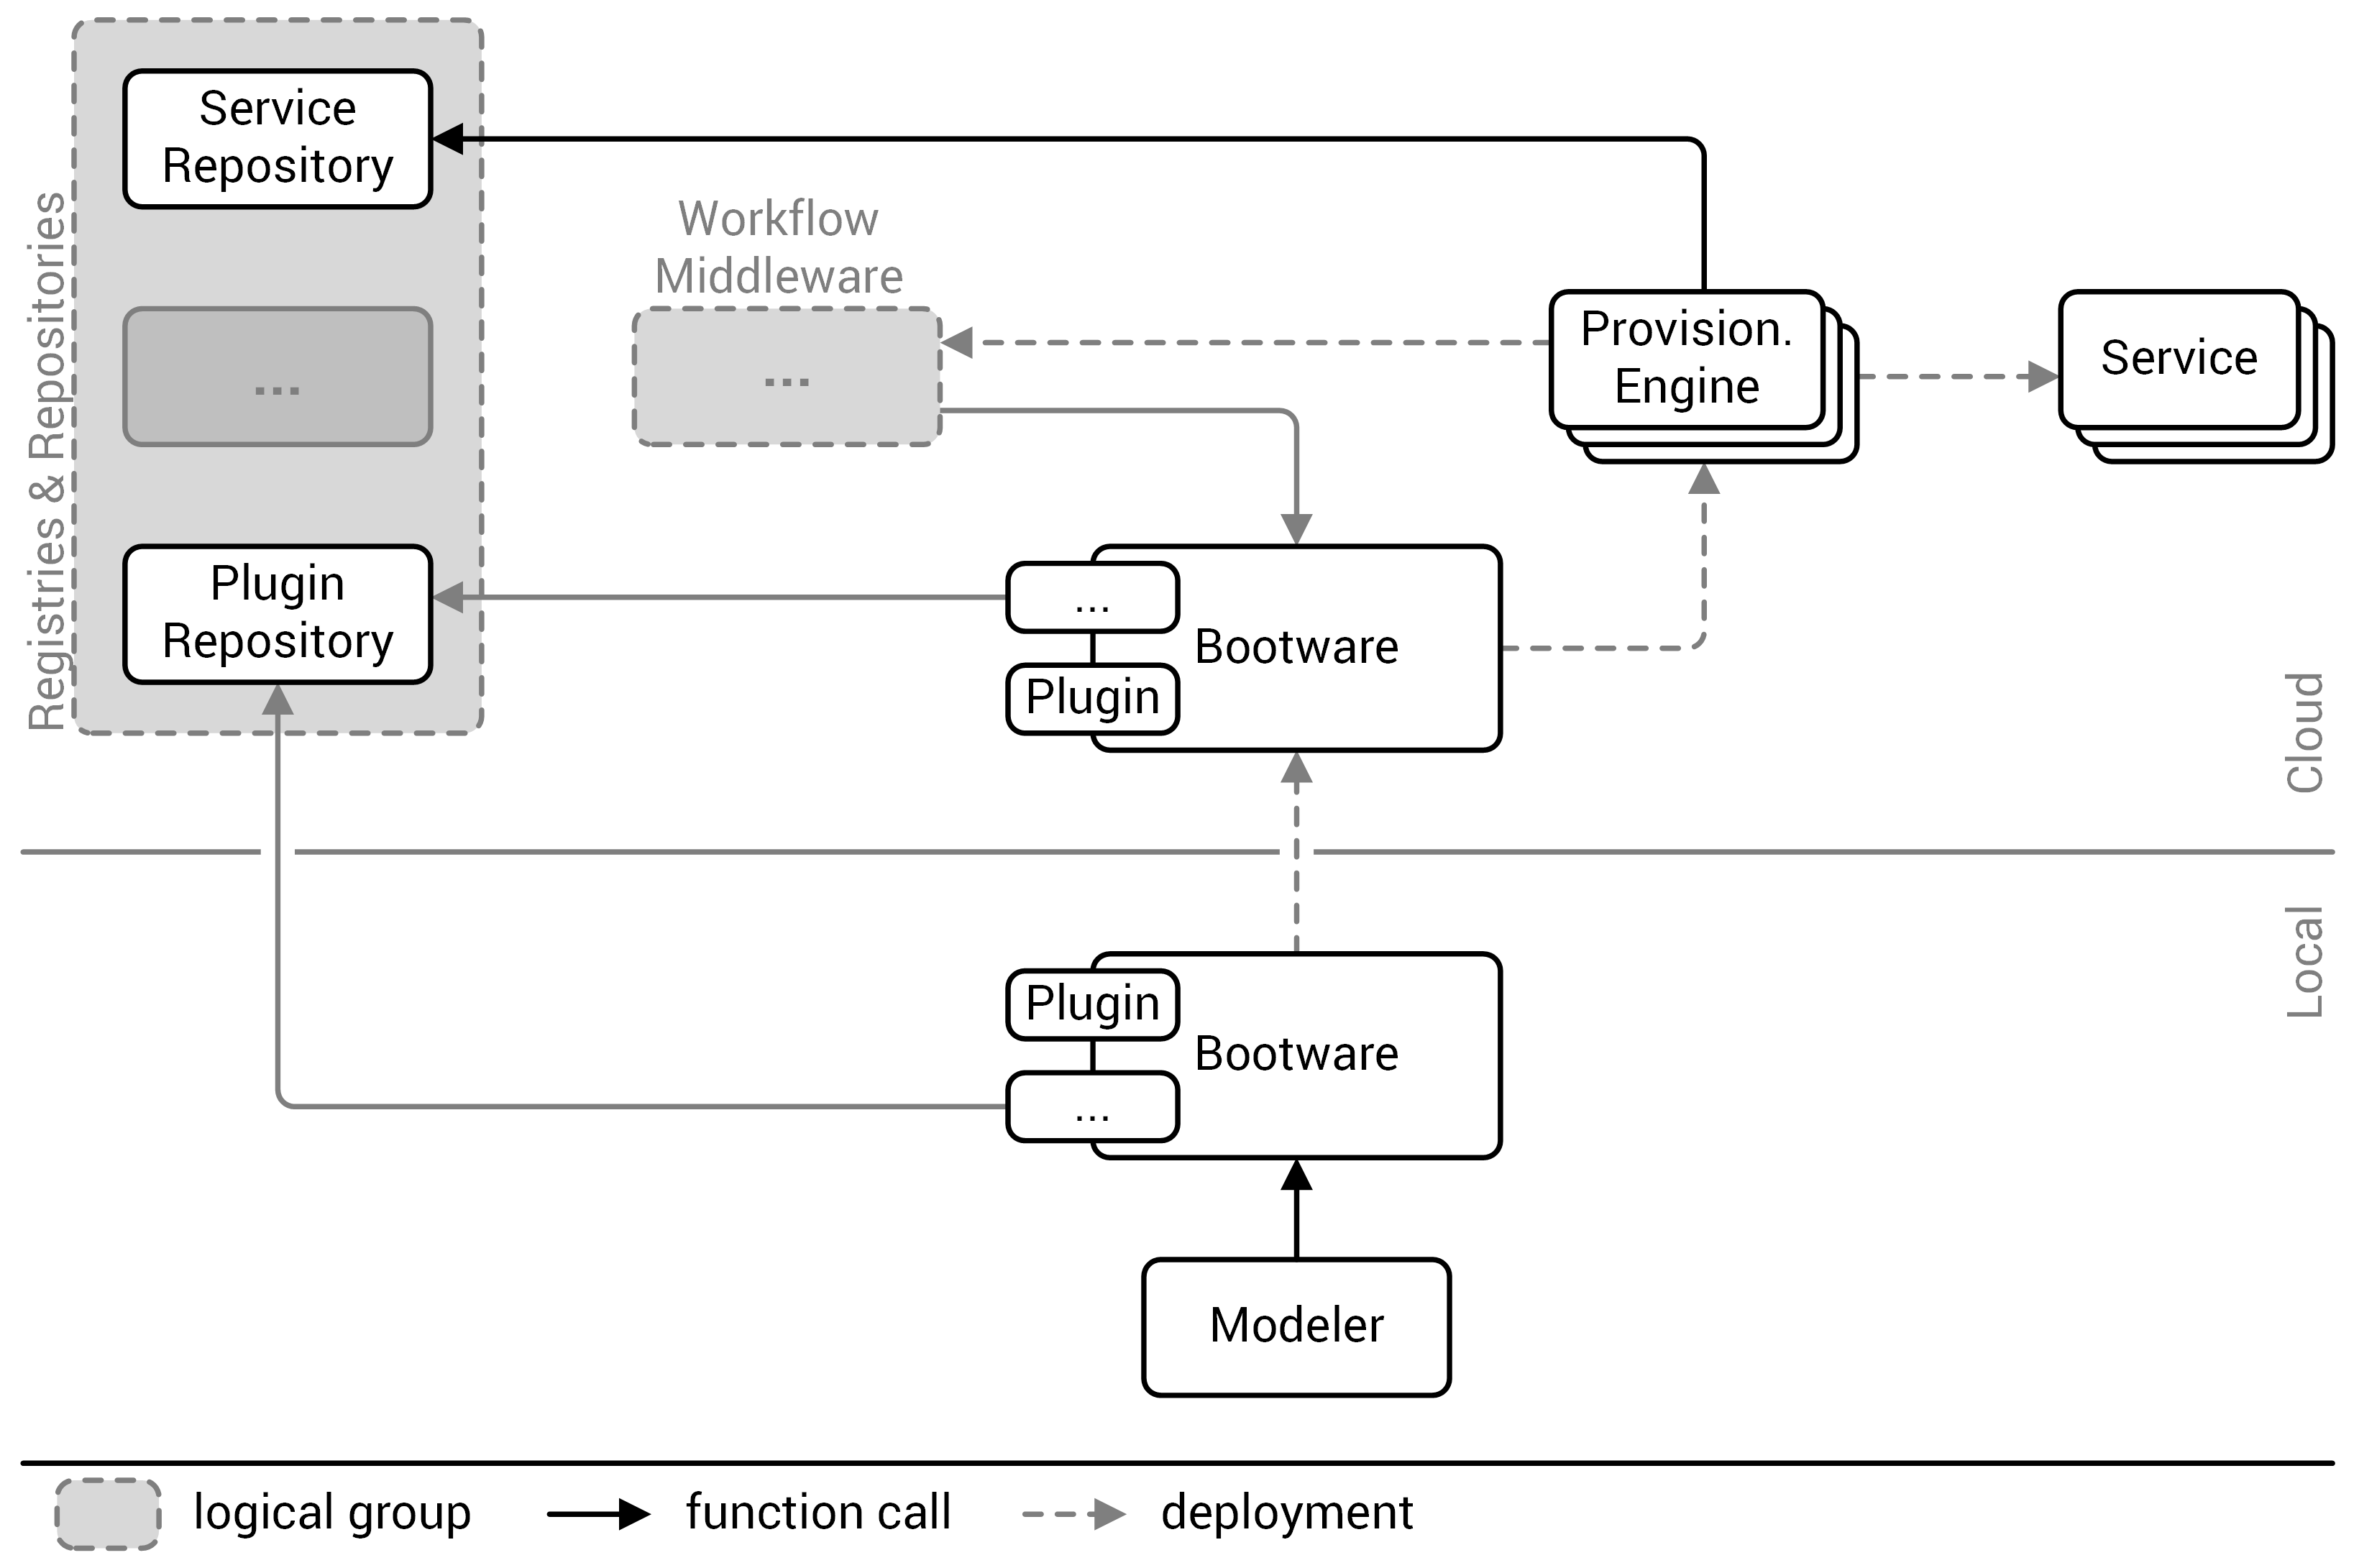
\includegraphics[resolution=600]{design/assets/plugin_repository}
	\caption{Simplified overview of the 2-tier architecture with a plugin repository.}
	\label{image:plugin_repository}
\end{figure}

\section{External Communication}
\label{design:communication}

In \autoref{design:modeler_integration} we established that a bootware plugin in the modeler has to call the local bootware.
From \autoref{design:division} we also know that both the local bootware and the provisioning manager have to call the remote bootware.
We now have to decide, how this external communication with the bootware will work.
There are several factors that impact this decision.
Communication between the components should be as simple as possible, but has to support some critical features.
To keep it simple, it would make sense to use the same communication mechanism for communication between the bootware components as well as with other external components, like the provisioning manager and the modeler plugin.

Since the provisioning processes kicked off by the bootware can potentially take a long time to finish (in the range of minutes to hours), asynchronous communication should be used between the components to avoid timeouts and blocking resources.
For the same reason, there should be some mechanism to get feedback on the current status during a long running provisioning process.

The communication with the bootware components will contain sensitive data, for example login information for cloud providers.
This information has to be provided from the outside and should be transported securely to prevent malicious or fraudulent attacks.
The selected communication method therefore has to support some sort of security mechanism, ideally end-to-end encryption.
While these security mechanisms will not be used in this thesis due to time constraints, selecting the right communication method is still critical for future development.

Java provides a package for \nom{Remote Method Invocation}{RMI}\footnote{\url{http://docs.oracle.com/javase/7/docs/api/java/rmi/package-summary.html\#package_description}}, which allows objects in one Java VM to invoke methods on objects in another Java VM.
But since RMI is limited to Java and we might want to communicate with the bootware from a component written in another programming language, RMI doesn't seem like a good fit.
For communication between programs written in different languages we could use the \nom{Common Object Request Broker Architecture}{CORBA}, a standard defined by the \nom{Object Management Group}{OMG}.
It supports mappings for common programming languages, like Java, C++, Python, and others.
CORBA also supports asynchronous method invocation via callbacks~\autocite{corba:async} and transport layer encryption and other security features~\autocite{corba:security}.

As a second alternative, we could communicate with messages by using message-oriented middleware.
As explained earlier in \autoref{fundamentals:service}, it supports communication between different components using adapters and channels.
Asynchronous communication is supported by using message queues for temporary storage.
The middleware can also provide additional persistent storage and backups for high availability~\autocite{mom}.
It may also support security features like encryption.
Another alternative are web services via \nom{Simple Object Access Protocol}{SOAP} or \nom{Representational State Transfer}{REST}.
Like CORBA, web services also support asynchronous invocation, as well as security mechanisms~\autocite{ws:security}.

\begin{figure}[!htbp]
	\centering
	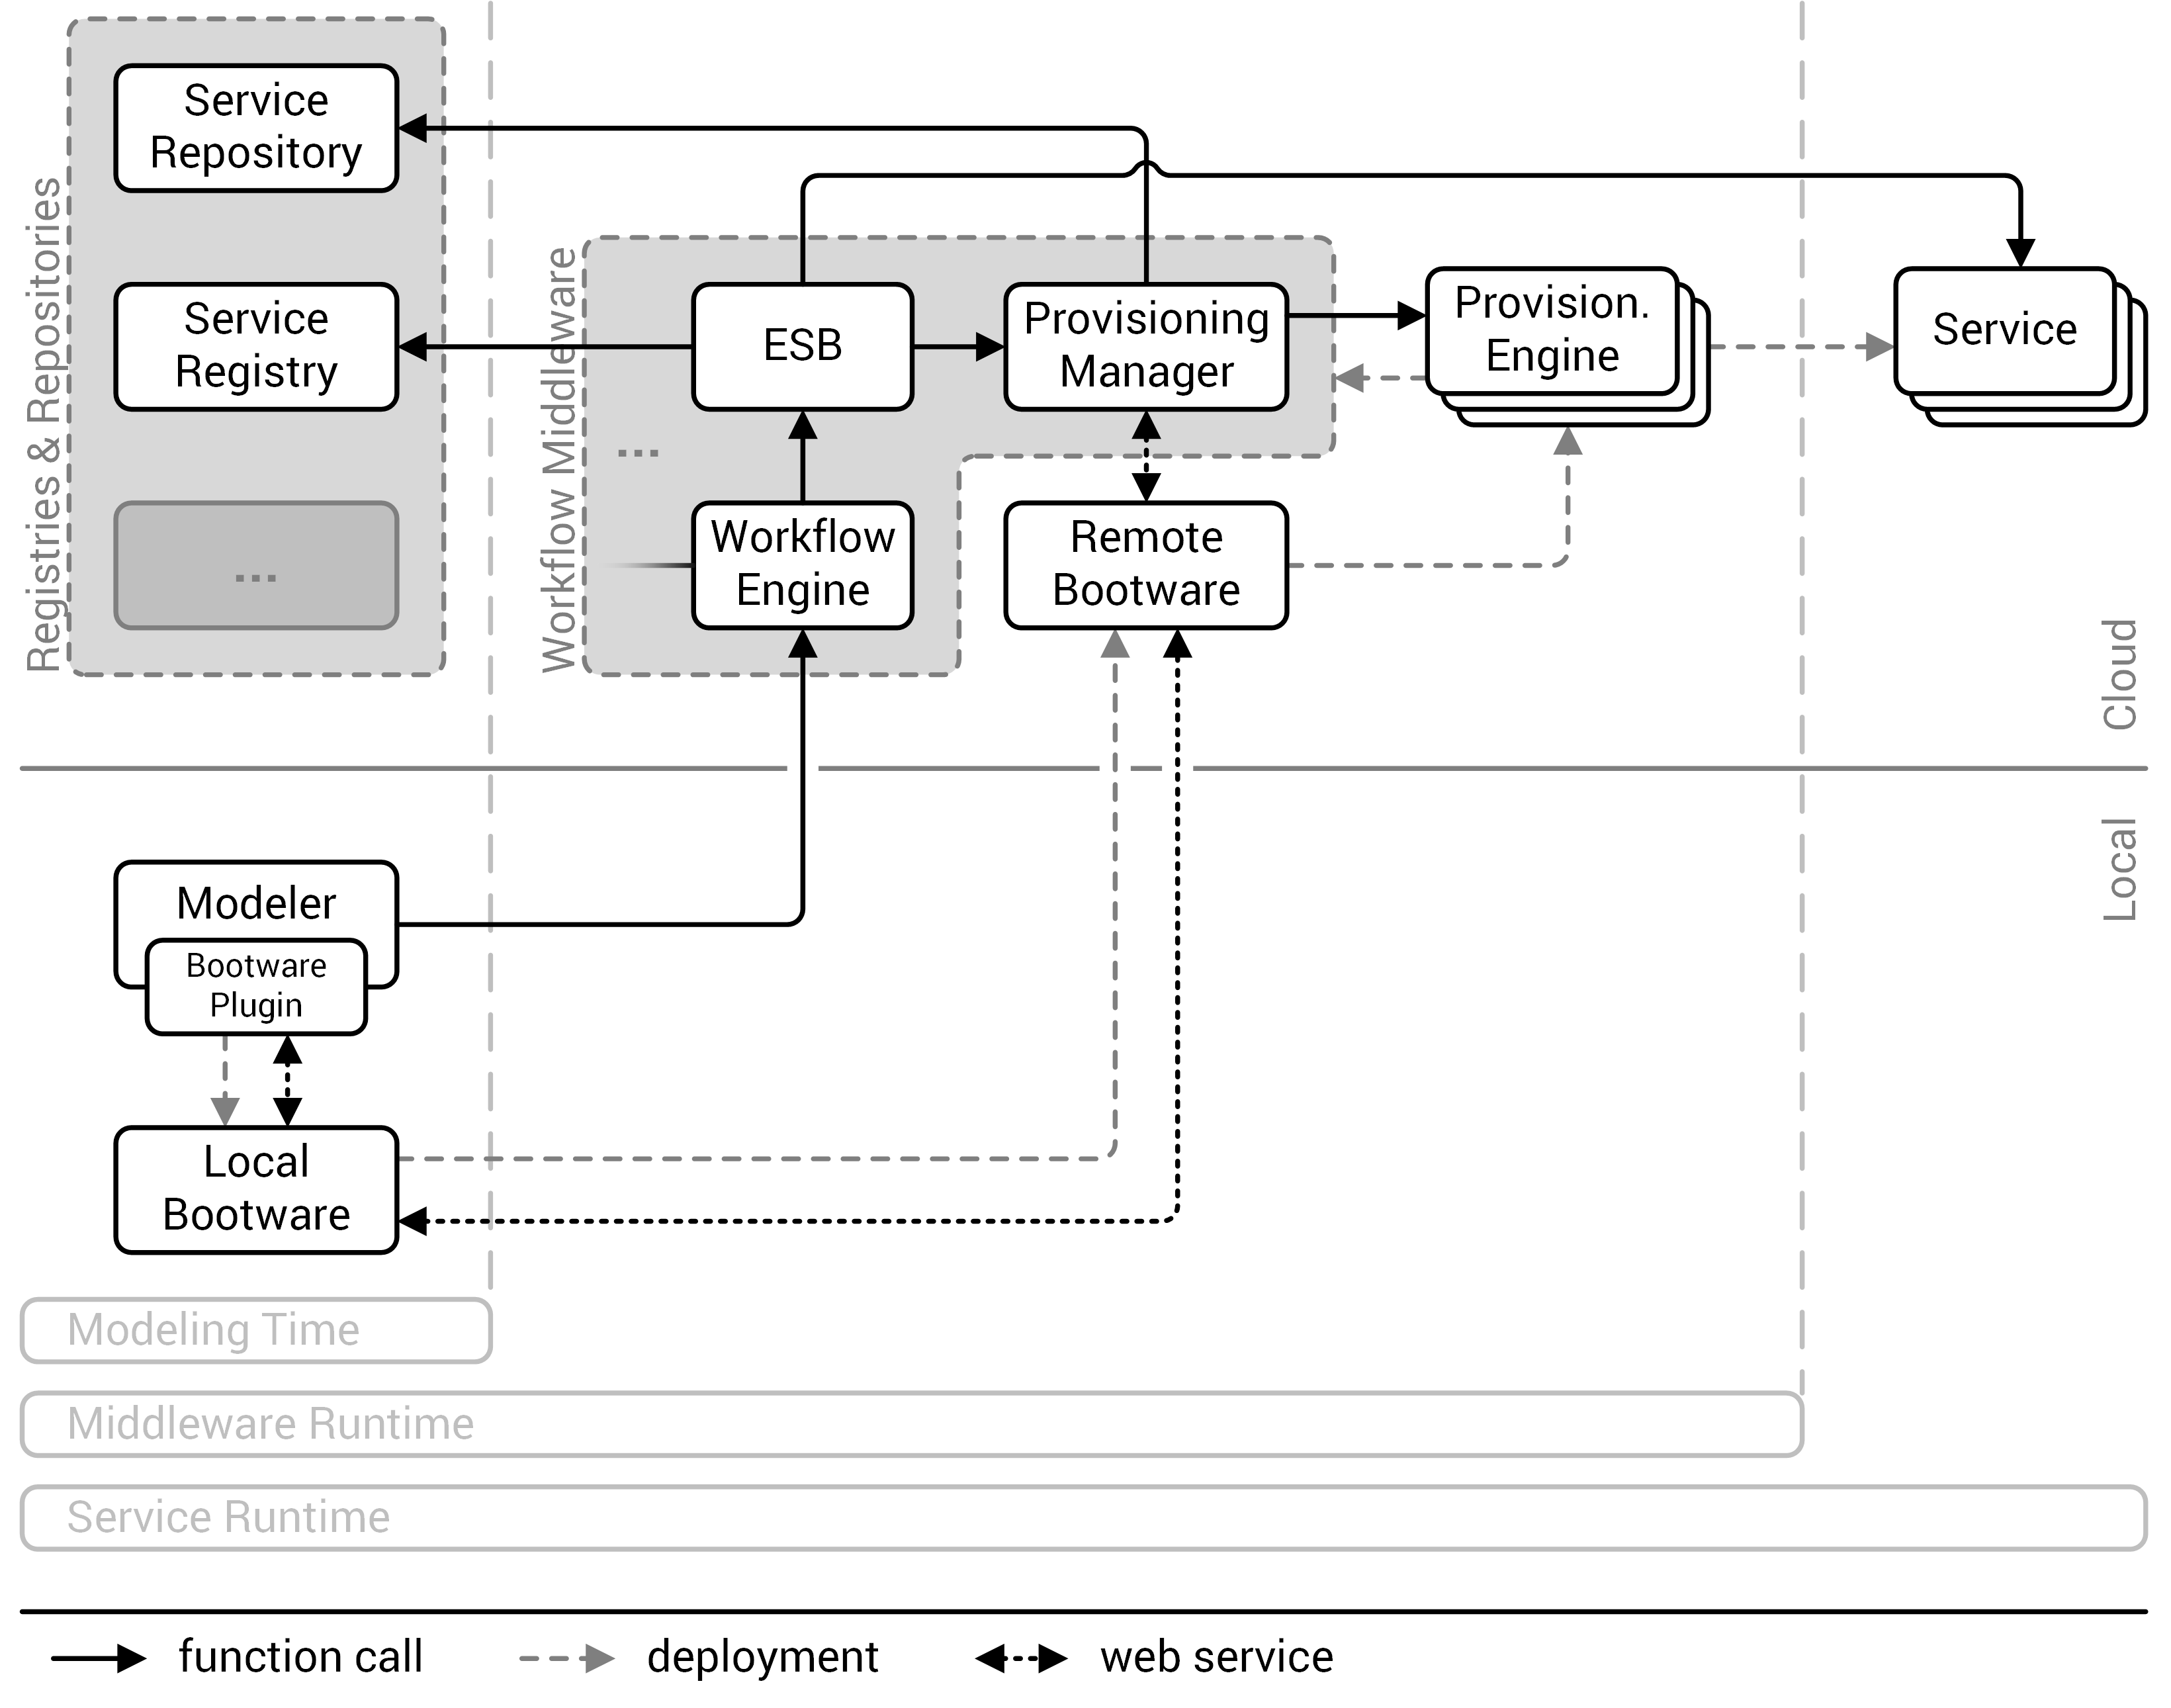
\includegraphics[resolution=600]{design/assets/webservice}
	\caption{Simplified overview of the 2-tier architecture with asynchronous web service communication}
	\label{image:webservice}
\end{figure}

Since the whole SimTech SWfMS already uses SOAP based web services, it would make sense to also use SOAP based web services as external communication mechanism for the bootware.
The technology and knowledge is already in place and introducing a second mechanism like CORBA would unnecessarily increase the complexity of the project, especially since CORBA doesn't offer any significant advantages over SOAP based web services.
\autoref{image:webservice} shows the addition of asynchronous web service call and return communication between the modeler bootware plugin and the local bootware, and between the remote bootware and the local bootware, as well as the provisioning manager.

With asynchronous communication, long running provisioning processes won't pose a problem.
We do however still need information during those long running processes to give the user some feedback.
This can't be accomplished by the simple web service request/response pattern.
For this, a secondary communication mechanism which supports sending multiple feedback messages has to be used.

\begin{figure}[!htbp]
	\centering
	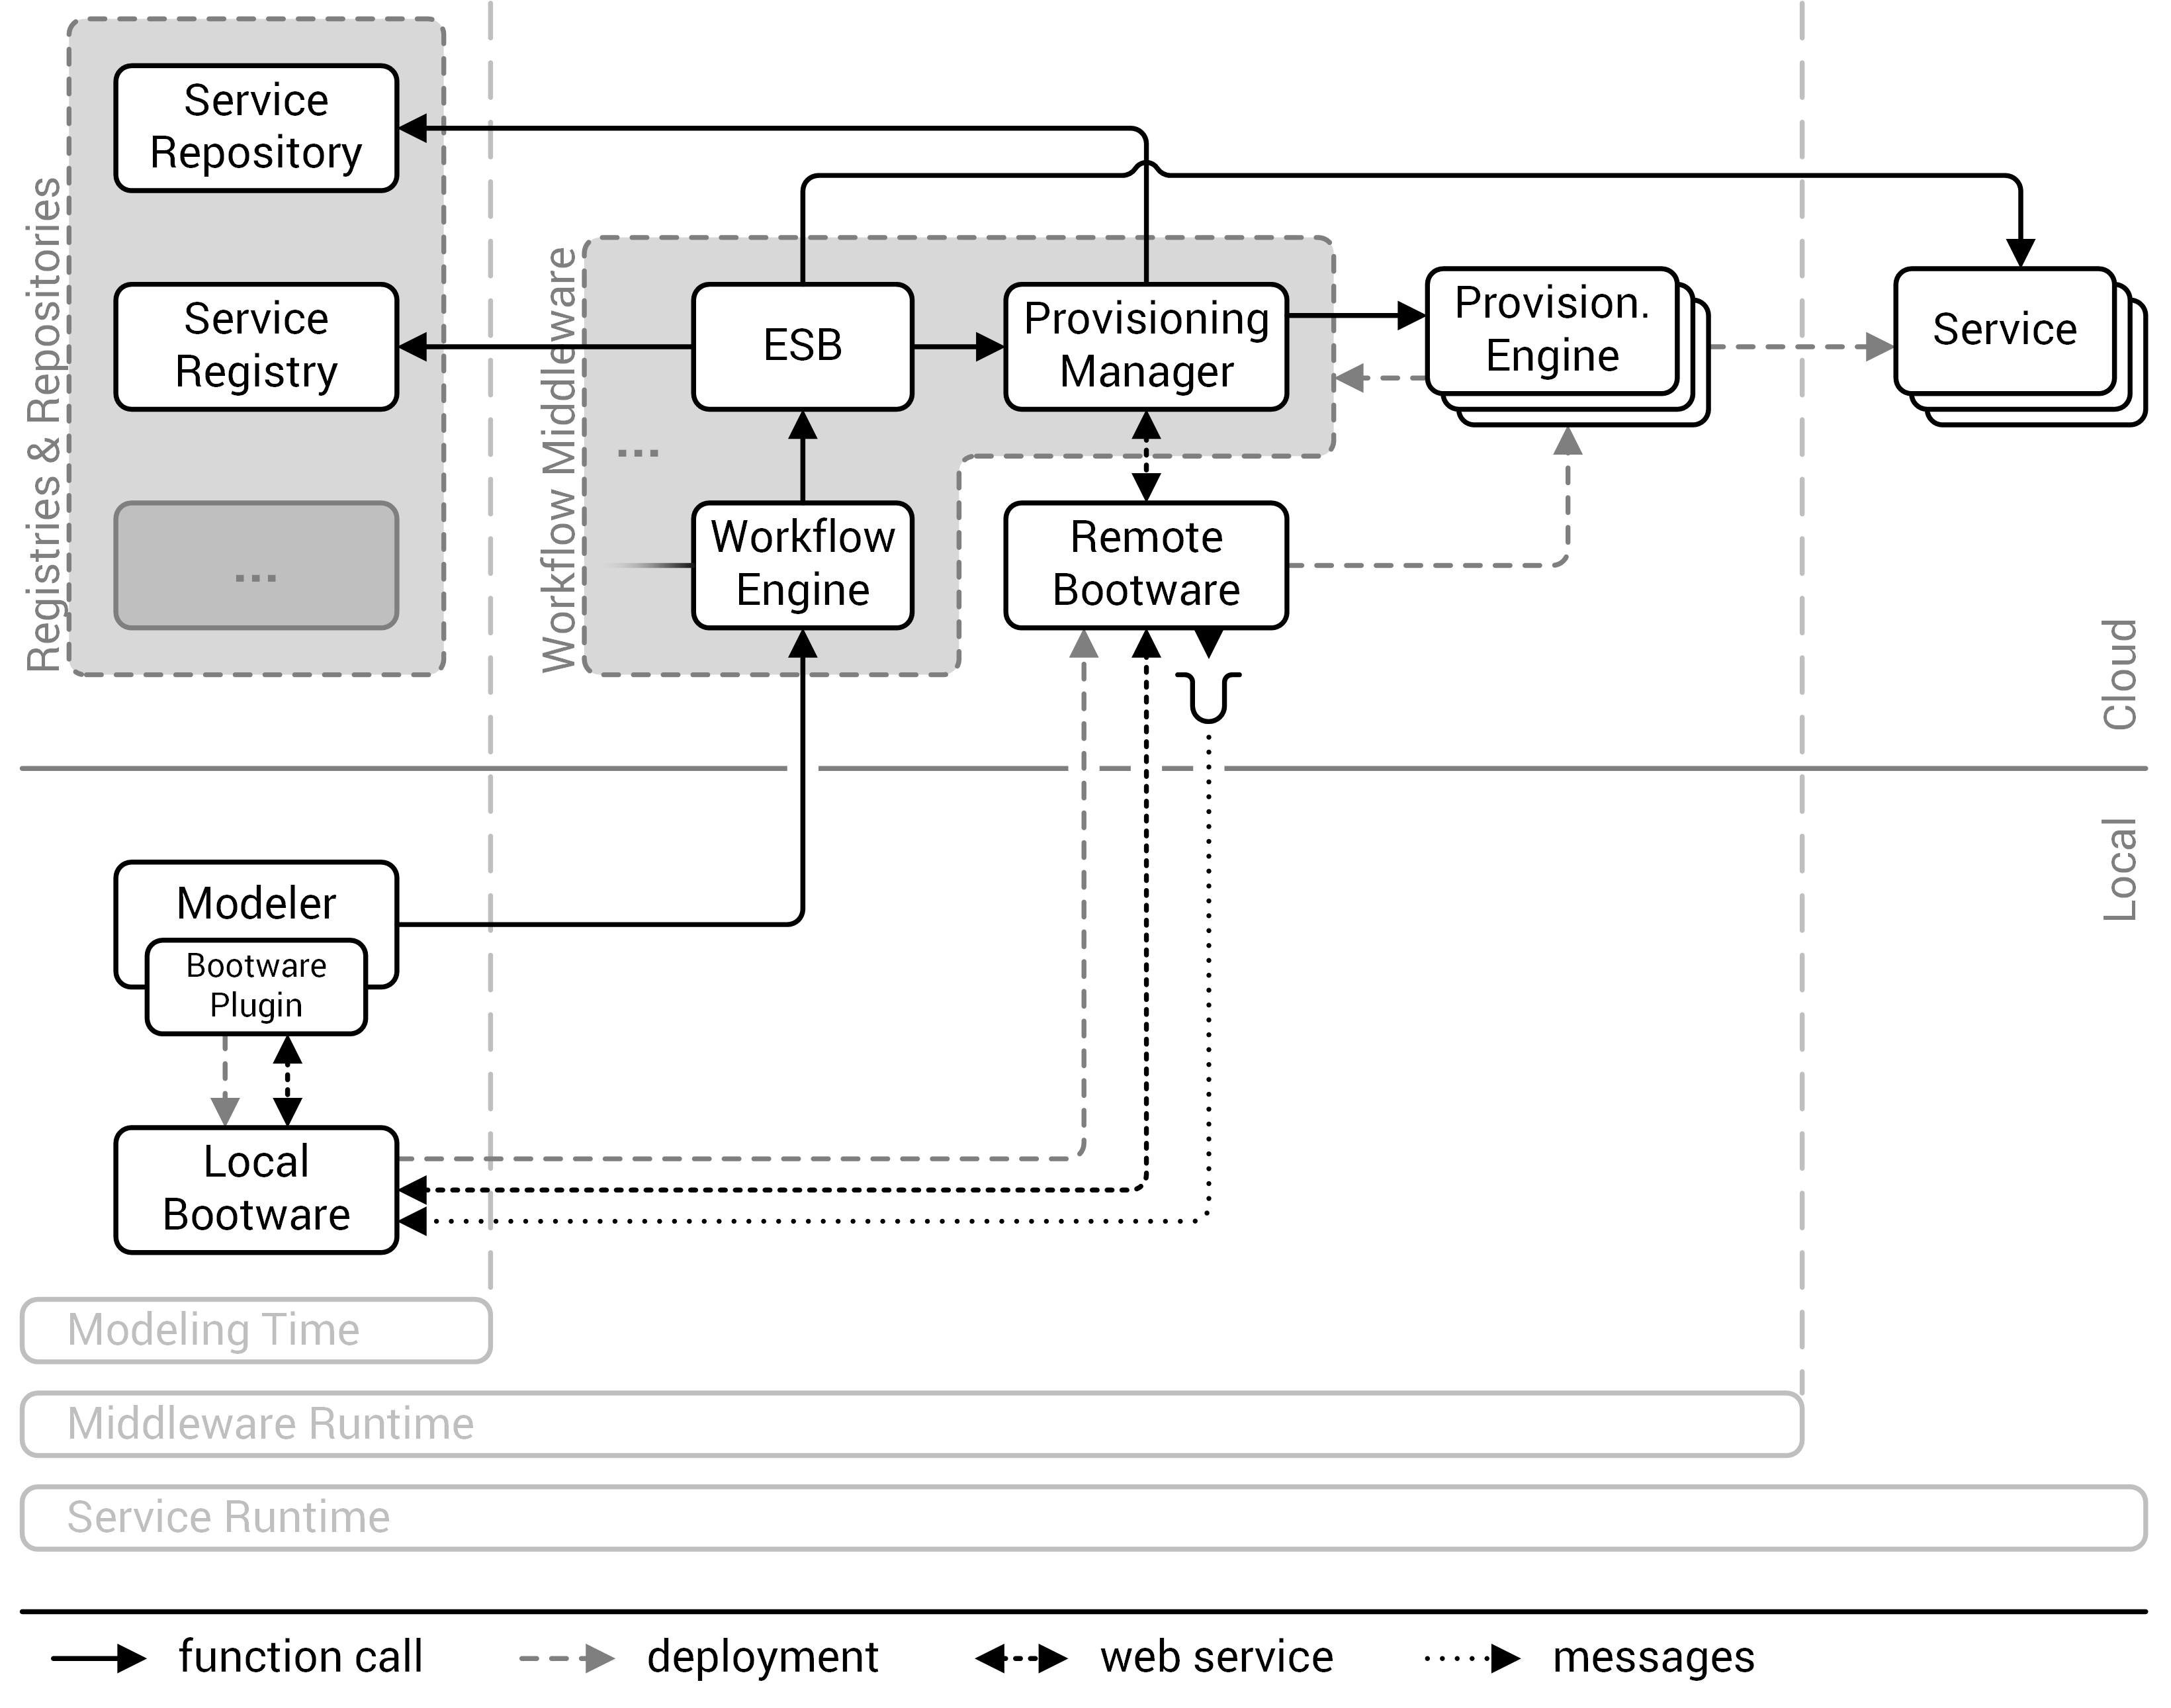
\includegraphics[resolution=600]{design/assets/message_queue}
	\caption{Simplified overview of the 2-tier architecture with asynchronous web service and messaging queue communication}
	\label{image:message_queue}
\end{figure}

This secondary communication channel could take any form, but a natural choice for publishing the intermediary state of the bootware would be a message queue system.
In this case, the remote bootware pushes messages to a message queue to which the local bootware (and other components if needs be) can subscribe to receive future messages.
\autoref{image:message_queue} shows the proposed architecture with an additional (and optional) message queue that allows the local bootware or other components to listen to status updates from the remote bootware.
Since it is not necessary for the successful use of the bootware, it would make sense to implement this secondary communication mechanism as an extension to the bootware.
This extension would not be part of the core bootware, but rather an additional component that could be used when needed.
This would allow us to add arbitrary communication extensions to the bootware depending on future needs.
How this can be done will be discussed in the next section.

\section{Internal Communication}
\label{design:internalcomm}

We also have to consider internal communication between the bootware core and plugins, and possibly also in between plugins.
Ideally, every plugin will be able to react to events from the bootware.
These events could be triggered by the bootware core or by any plugin, but plugins should be completely independent from each other.
Since a plugin does not know about other plugins, it can not listen for events at other plugins directly.
The only known constant to a plugin is the bootware core.
Therefore we need a communication mechanism which allows for loosely coupled communication between the bootware core and the plugins, where plugins can register their interest for certain events with the core and also publish their own events to the core for other plugins to consume.
This essentially describes the publish-subscribe pattern~\autocite{pubsub}.

\subsection{Publish Subscribe Pattern}

The \nom{publish-subscribe pattern}{PubSub} is a messaging pattern that consists of three types of participant: An event bus (or message broker), publishers, and subscribers.
The event bus sits at the center of the communication.
It receives messages from publishers and distributes them to all subscribers that have voiced their interest in messages of a certain type by subscribing at the event bus~\autocite{pubsub}.
Using this pattern, we would create an event bus at the bootware core and plugins, as well as other parts of the core, could subscribe at this event bus and also publish messages through this event bus.

\begin{figure}[!htbp]
	\centering
	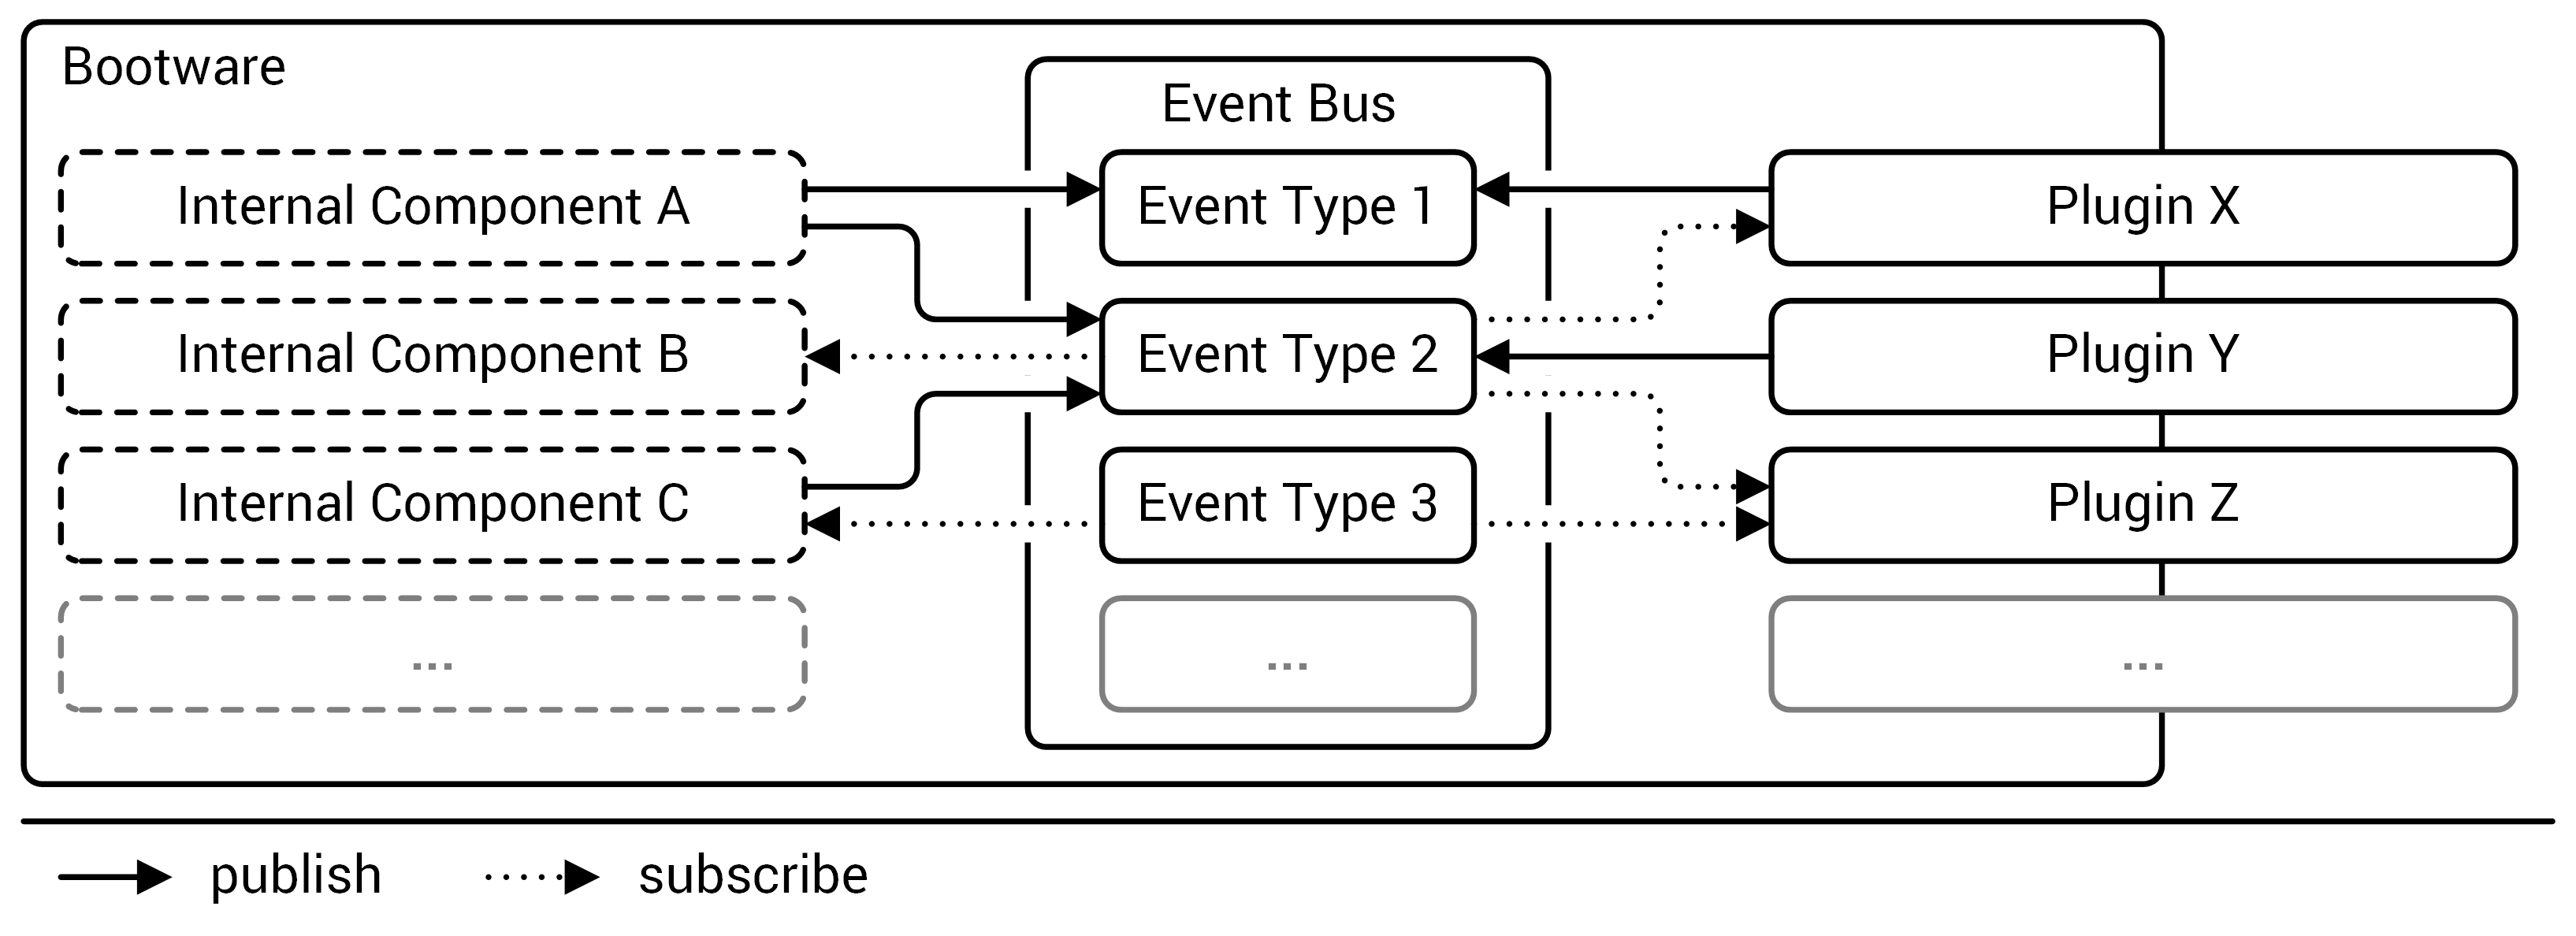
\includegraphics[resolution=600]{design/assets/pubsub}
	\caption{Bootware internal communication with PubSub pattern.}
	\label{image:pubsub}
\end{figure}

\subsection{Event Types}

When using PubSub and events to communicate, it is usually a good idea to not only use one type of event, but many different types.
Using different kinds of event allows us to subscribe only to specific events or react differently based on the type of an event.
But what if we want to react to each event type in the same way, for example for logging purposes?
Now, many different event types complicate things more.
This is where event hierarchies become useful.
At the core of an event hierarchy is a single base event.
By extending and refining this base event, other, more specific event types can be created, which again can be used as base type for even more specific events.
This allows us to create a fine grained hierarchy of events and also enables us to subscribe to particular sub sets of this hierarchy.
This makes event handling much easier, since we can now just react to the parent event if we do not need to distinguish between different event types for a particular task.

A second mechanism to differentiate between events is some sort of severity value that each event contains.
Many events will be published in an event system, but not all of them might be of the same importance.
The majority might be of low value while a few events might be very important.
For example, for logging purposes we might not be interested in every event, but only warnings and errors.
By adding a severity attribute to the base event type, all events could be categorized in different severity groups and filtered accordingly if needed.
As we can see, we might benefit from a well thought-out event hierarchy.

\vspace*{\baselineskip}
\begingroup
	\centering
	\captionsetup{type=figure}
	\begin{description}
		\item[BaseEvent] on which all other events are based
		\begin{description}
			\item[CoreEvent] published by the bootware core
			\begin{description}
				\item[PluginManagerEvent] for loading and unloading plugins
				\begin{description}
					\item[PluginLoadEvent] could be info, success, warning, or error
					\item[PluginUnloadEvent] could be info, success, warning, or error
					\item[\ldots] ~
				\end{description}
				\item[\ldots] ~
			\end{description}
		\end{description}
		\begin{description}
			\item[PluginEvent] published by a plugin
			\begin{description}
				\item[InfrastructurePluginEvent] contains further child events defined by plugin
				\item[ConnectionPluginEvent] contains further child events defined by plugin
				\item[PayloadPluginEvent] contains further child events defined by plugin
				\item[EventPluginEvent] contains further child events defined by plugin
				\item[\ldots] ~
			\end{description}
		\end{description}
	\end{description}
	\caption{Exemplary event hierarchy.}
	\label{figure:eventhierarchy}
\endgroup

\autoref{figure:eventhierarchy} shows an exemplary event hierarchy for the bootware.
As we can, every event is based on the BaseEvent, shown at the top.
Events can be further divided into core events that are published by the bootware core and plugin events that are published by plugins.
Core events contain events from the various core components of the bootware, for example the plugin manager.
The plugin manager events are further divided into events for certain operation that can also have different severity values (i.e. info, success, warning, and error).
Plugin events are divided by plugin types.
Different plugins can also add further child events to these event types.

